\begin{example}[Advection-diffusion 2D]
\label{ex:quart3}
Based on Example 3 in \cite{Antonietti2013},
in $\Omega = [0, 1]^2$ we will once again solve the equation \eqref{eq:ex_advdiff}
%\begin{equation}
%	\pdiff{u}{x} + \pdiff{u}{y} - D \cdot \left( \pdiff{^2 u}{x^2} + \pdiff{^2
%	u}{y^2} \right) = g
%\end{equation}
%i.e
%\begin{equation}
%	\vec{a} \cdot \nabla u - D \Delta u = g
%\end{equation}
%where $\vec{a} = [1, 1]^T$ is advection velocity and $D$ is diffusion
%coefficient and $g$ is a source function.
We set up the boundary condition and source function in such a way that the exact
solution $u_{exact}$ is
\begin{equation}
	u_{exact} = -xy + x +y + \frac{\exp{\left(-\frac{{\left(x - 1\right)} {\left(y -
	1\right)}}{D}\right)} -
	\exp{\left(-\frac{1}{D}\right)}}{\exp{\left(-\frac{1}{D}\right)}
	- 1}.
\end{equation}
We omit analytical forms of $g$ and boundary conditions for brevity, they can found in
the code. Different values of the coefficient $C_w$ in the penalty term yield different
convergence behavior as demonstrated in Figures \ref{fig:orders_quarteroni3} and 
\ref{fig:conv_qart3}. Antonietti et al. \cite{Antonietti2013} report convergence
for order 1 and 2, these are in accord with ours. \todo

\begin{figure}[h!]
    \centering
    \begin{subfigure}{.5\textwidth}
        \centering
        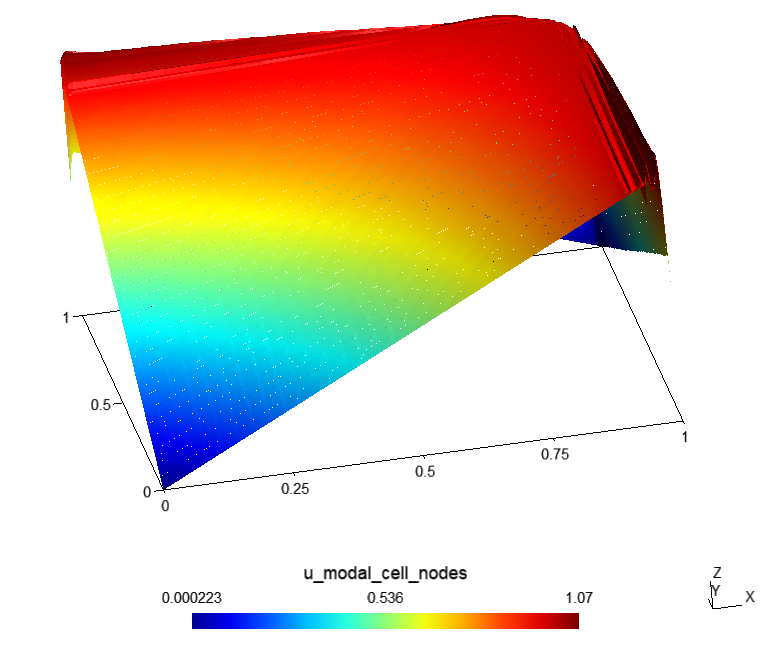
\includegraphics[width=.8\linewidth]{../figs/sols/quart3-00000-sol-h1024o04}
        \caption{$C_w = 1$}
    \end{subfigure}%
    \begin{subfigure}{.5\textwidth}
        \centering
        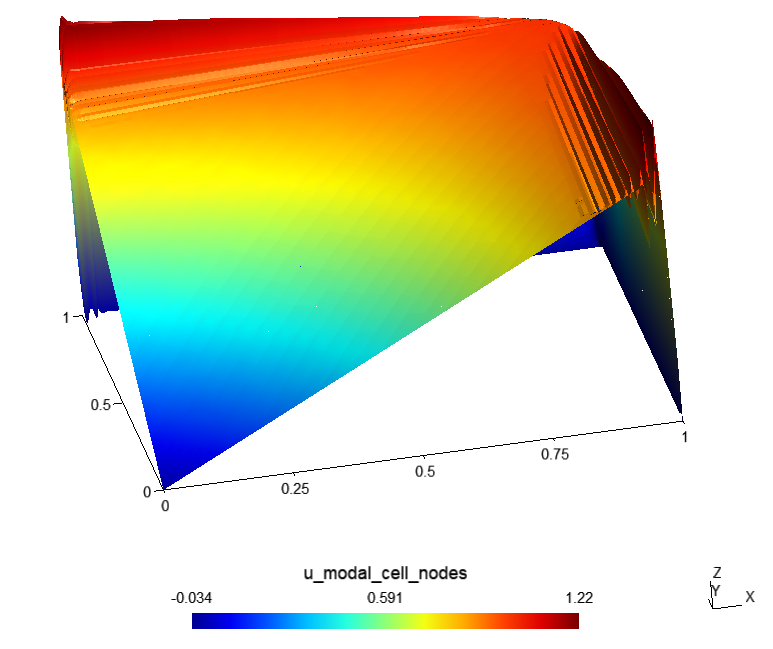
\includegraphics[width=.8\linewidth]{../figs/sols/quart3-30000-sol-h1024o04}
        \caption{$C_w = 10^3$}
    \end{subfigure}
    \caption{\Cref{ex:quart3}. Solutions using quadrilateral mesh for $D = 0.001$ and
        for different values of $C_w$ for quadrilaterals (left) and triangles (right).}
    \label{fig:sol_quart3}
\end{figure}


\begin{figure}[h!]
    \centering
    \begin{tabular}{p{0.5\textwidth} p{0.5\textwidth}}
        \vspace{0pt}
        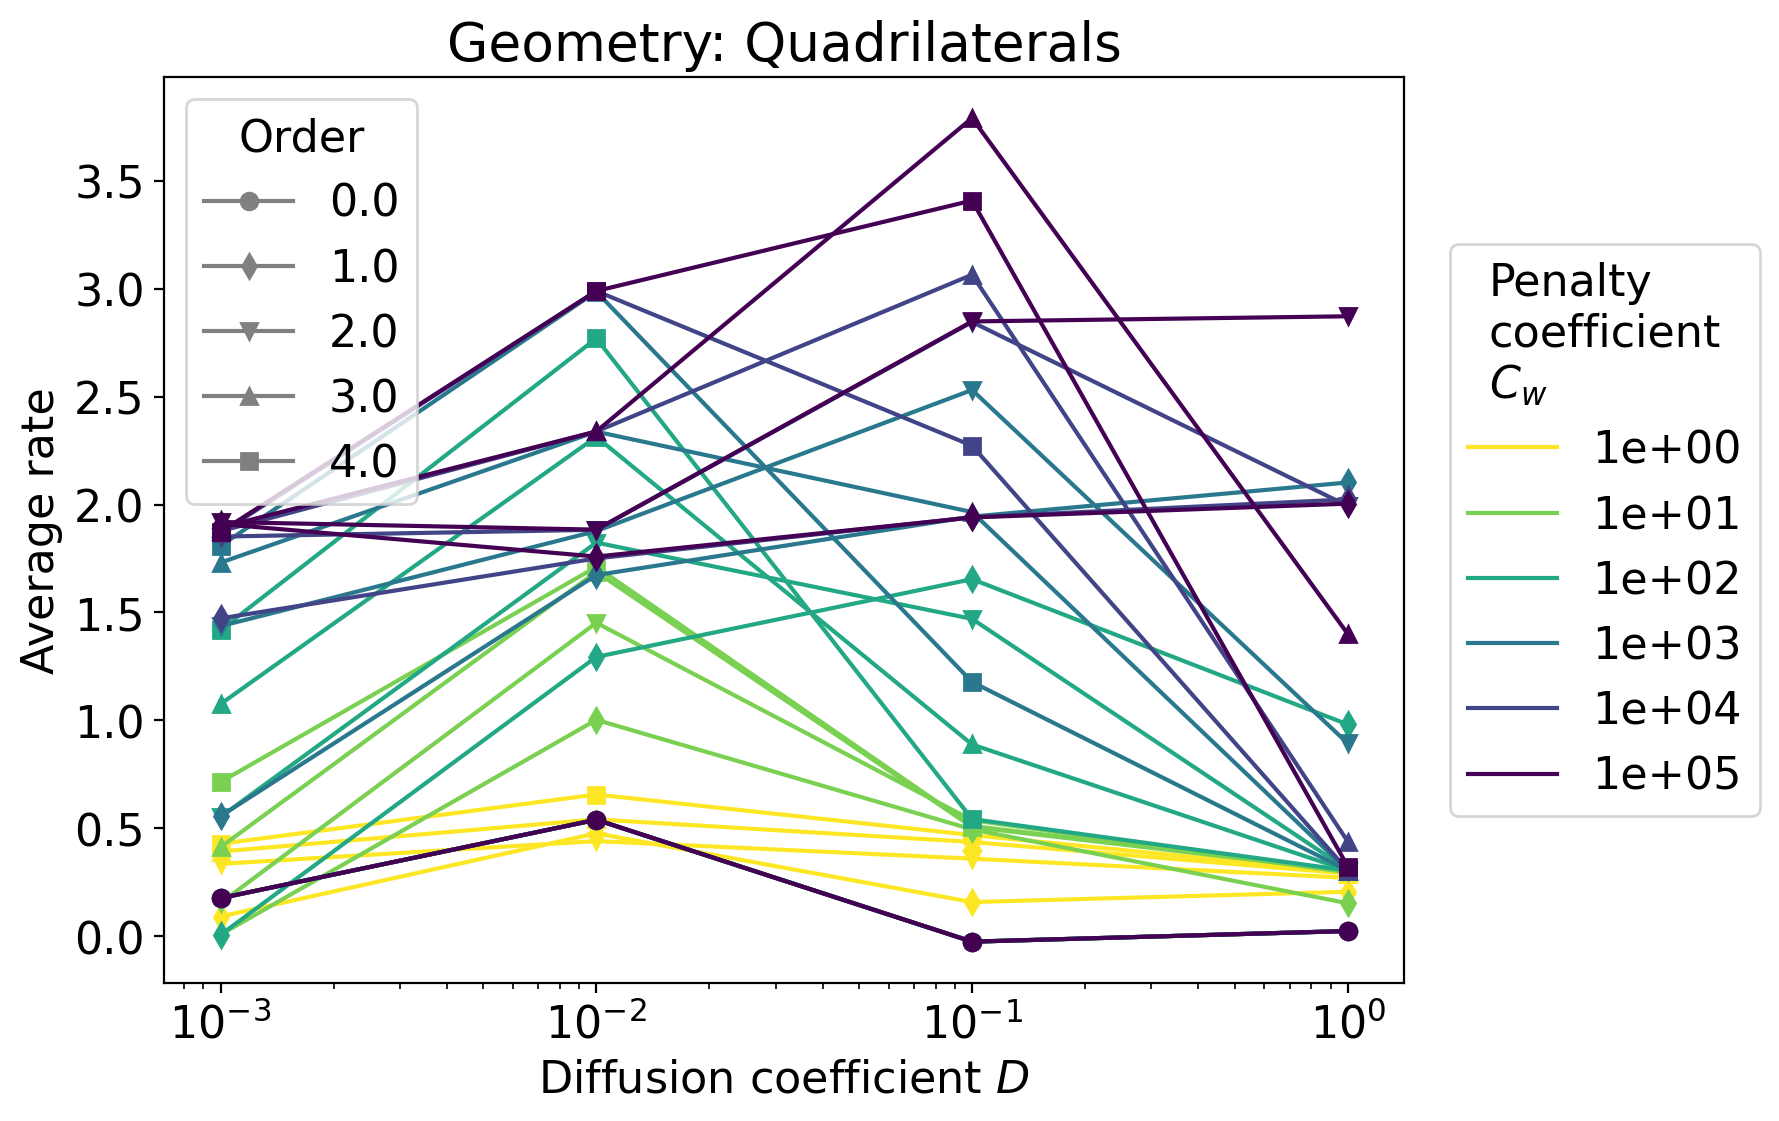
\includegraphics[width=0.5\textwidth]{../figs/parametric/advdiff_2D/ord_quarteroni3_2_4}
        &
        \vspace{0pt}
        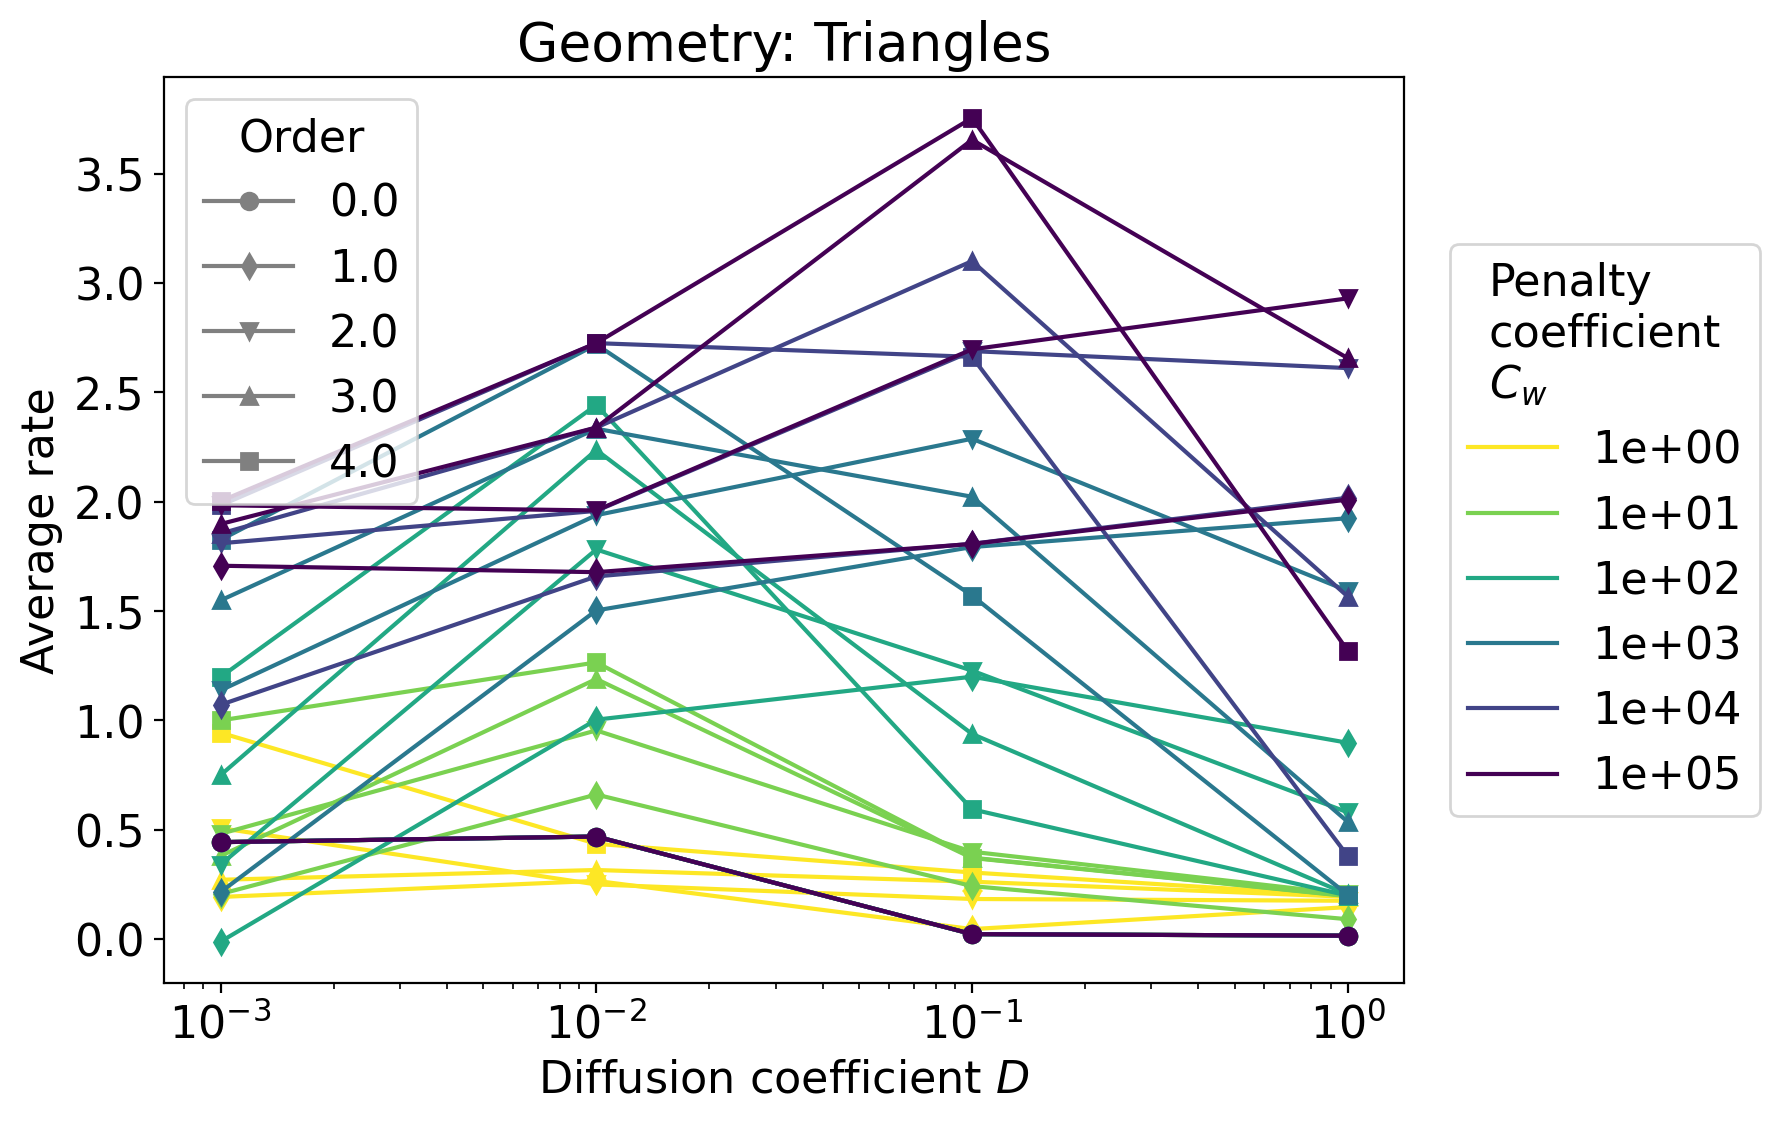
\includegraphics[width=0.5\textwidth]{../figs/parametric/advdiff_2D/ord_quarteroni3_2_3}
    \end{tabular}
    \caption{\Cref{ex:quart3}. Average convergence rate for different choices of $C_w$}
    \label{fig:orders_quarteroni3}
\end{figure}
\end{example}


\begin{figure}[p!]
	\centering
	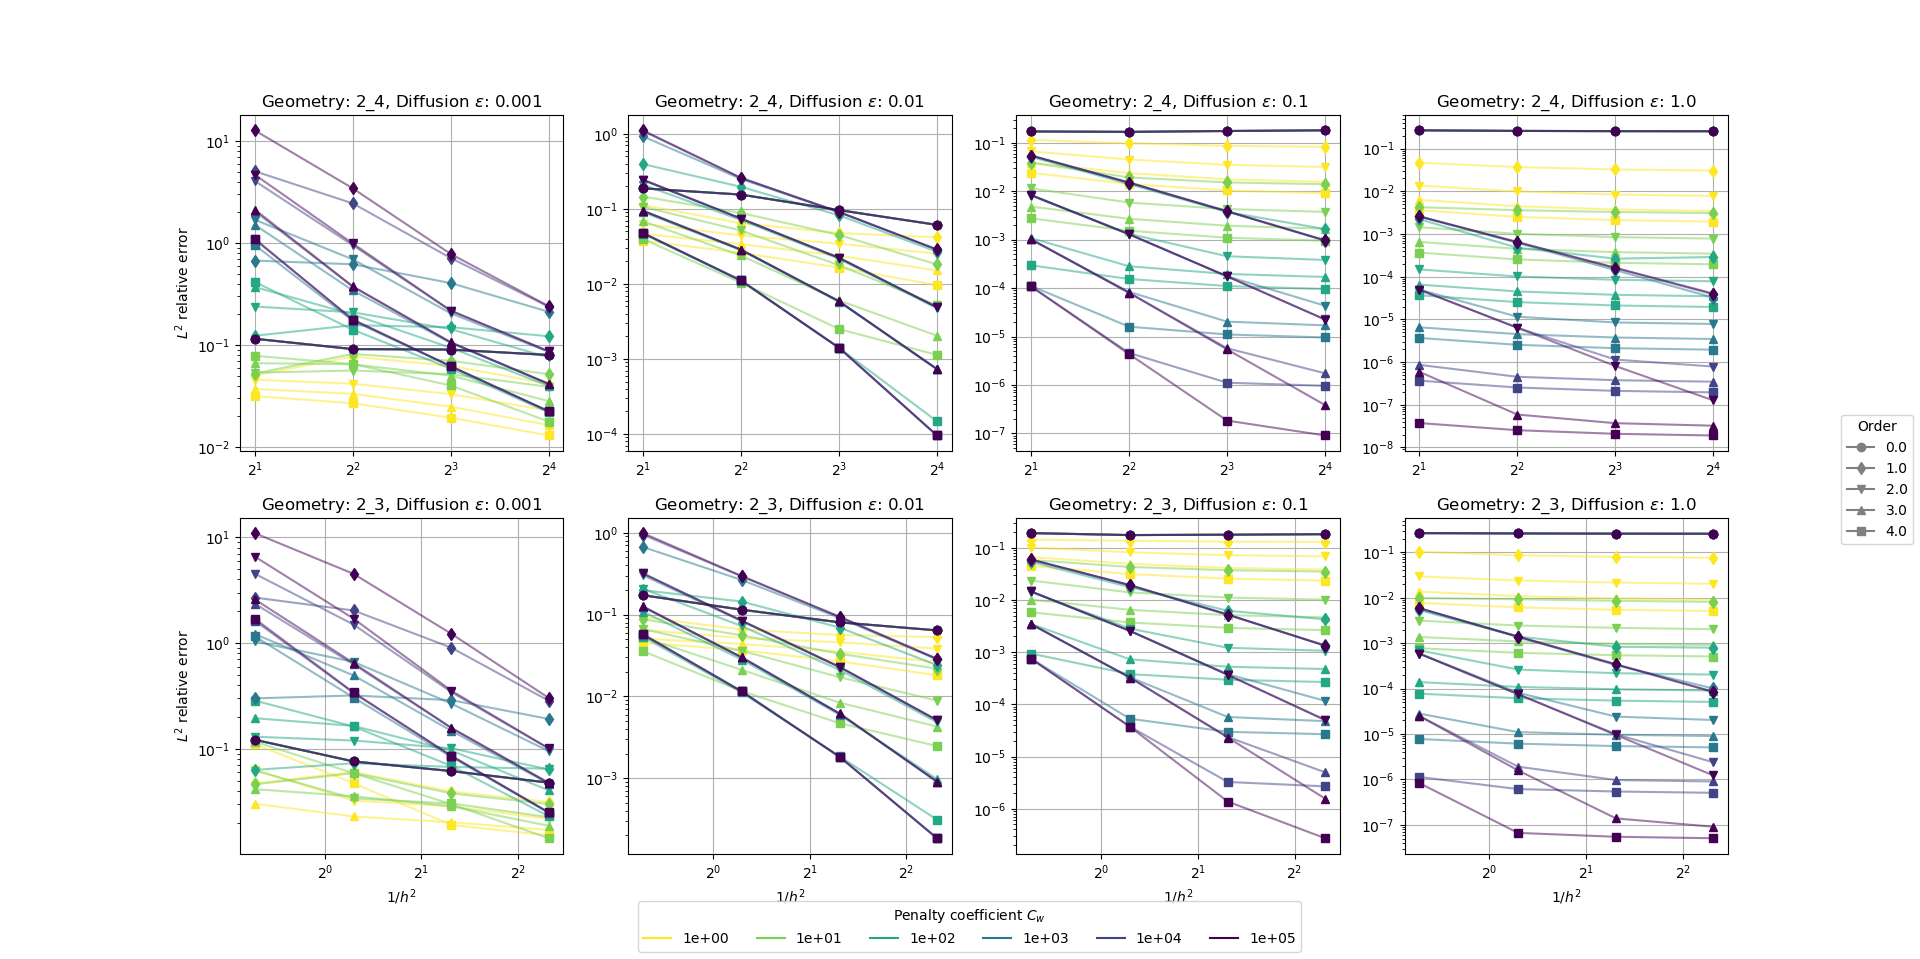
\includegraphics[height=\textheight]{../figs/parametric/advdiff_2D/quarteroni3.png}

	\caption{\Cref{ex:quart3}. Relative errors for different choice of $C_w$ for
	quadrilaterals (left) and triangles (right).}
	\label{fig:conv_qart3}
\end{figure}